\documentclass{article}
\usepackage{tabularx,booktabs,geometry,graphicx,pdflscape}
\renewcommand\tabularxcolumn[1]{>{\Centering}p{#1}}
\geometry{a4paper,left=25mm,right=25mm,top=15mm,bottom=15mm}
{\def\sym#1{\ifmmode^{#1}\else\(^{#1}\)\fi}
	
\begin{document}
	
This document explains the empirical model we used. We used R to generate regression results because R has a package (stargazer) that formats regression output into tables that we show below. The following tables and graphs are all generated from R code.

\bigskip

For Table 1, we run the following model:
$$
Salary_i = \gamma StateCharacterstics_j + \epsilon_i
$$
where each unit of observation i is a job posting on glassdoor, and $StateCharacterstics_j$ is a state-level variable. We add variables incrementally.

\bigskip \bigskip

For Table 2, we run the following model:
$$
Salary_i = \gamma StateCharacterstics_j + \delta CompanyCharacteristics_k + \epsilon_i
$$
where each unit of observation i is a job posting on glassdoor, $StateCharacterstics_j$ are state-level variables, and $CompanyCharacterics_k$ are company-level variables. We add variables incrementally.

\bigskip \bigskip

For Table 3, we run the following model:
$$
Salary_i = \gamma StateCharacterstics_j + \delta CompanyCharacteristics_k + \beta JobCharacteristics_i + \epsilon_i
$$
where each unit of observation i is a job posting on glassdoor, $StateCharacterstics_j$ are state-level variables, $CompanyCharacterics_k$ are company-level variables, and $JobCharacteristics_i$ are job-posting-level variables. We add variables incrementally.

\bigskip\bigskip
We then plot the residuals against state-level variables including Monthly Median Owner Cost, Percentage Employed in Tech, and Percentage With College Degree for selected models (Table 1 Col 6, Table 2 Col 6, and Table 3 Col 2). We also plot the distribution of residuals for these selected models.
	
	
	\begin{landscape}
		
% Table created by stargazer v.5.2.3 by Marek Hlavac, Social Policy Institute. E-mail: marek.hlavac at gmail.com
% Date and time: Mon, Mar 06, 2023 - 5:24:03 pm
\begin{table}[!htbp] \centering 
  \caption{Regressions on state level variables} 
  \label{} 
\footnotesize 
\begin{tabular}{@{\extracolsep{5pt}}lcccccc} 
\\[-1.8ex]\hline 
\hline \\[-1.8ex] 
 & \multicolumn{6}{c}{Dependent Variable: Annual Salary (in 1000s)} \\ 
\cline{2-7} 
\hline \\[-1.8ex] 
 Median Cost to Own a Home (Monthly) & 0.022$^{***}$ & 0.011$^{***}$ & 0.020$^{***}$ & 0.020$^{***}$ & 0.019$^{***}$ & 0.023$^{***}$ \\ 
  & (0.001) & (0.002) & (0.003) & (0.003) & (0.004) & (0.005) \\ 
  & & & & & & \\ 
 Percentage Employed in Tech &  & 11.200$^{***}$ & 12.000$^{***}$ & 12.500$^{***}$ & 12.700$^{***}$ & 13.000$^{***}$ \\ 
  &  & (1.760) & (1.760) & (1.870) & (1.900) & (1.910) \\ 
  & & & & & & \\ 
 Percentage of College Graduates &  &  & $-$0.800$^{***}$ & $-$0.870$^{***}$ & $-$0.930$^{***}$ & $-$0.962$^{***}$ \\ 
  &  &  & (0.153) & (0.176) & (0.206) & (0.207) \\ 
  & & & & & & \\ 
 Population (In Households) &  &  &  & $-$0.00000 & $-$0.00000 & $-$0.00000 \\ 
  &  &  &  & (0.00000) & (0.00000) & (0.00000) \\ 
  & & & & & & \\ 
 Median Income &  &  &  &  & 0.0001 & 0.0001 \\ 
  &  &  &  &  & (0.0001) & (0.0002) \\ 
  & & & & & & \\ 
 Median Rent (Monthly) &  &  &  &  &  & $-$0.010 \\ 
  &  &  &  &  &  & (0.006) \\ 
  & & & & & & \\ 
 Constant & 68.400$^{***}$ & 68.100$^{***}$ & 80.700$^{***}$ & 81.600$^{***}$ & 80.200$^{***}$ & 80.400$^{***}$ \\ 
  & (2.630) & (2.620) & (3.550) & (3.730) & (4.520) & (4.530) \\ 
  & & & & & & \\ 
\hline \\[-1.8ex] 
Observations & 4,409 & 4,409 & 4,409 & 4,409 & 4,409 & 4,409 \\ 
R$^{2}$ & 0.048 & 0.057 & 0.063 & 0.063 & 0.063 & 0.063 \\ 
\hline 
\hline \\[-1.8ex] 
\textit{Note:}  & \multicolumn{6}{r}{$^{*}$p$<$0.1; $^{**}$p$<$0.05; $^{***}$p$<$0.01} \\ 
\end{tabular} 
\end{table} 

	\end{landscape}

	\begin{landscape}
		
% Table created by stargazer v.5.2.3 by Marek Hlavac, Social Policy Institute. E-mail: marek.hlavac at gmail.com
% Date and time: Mon, Mar 06, 2023 - 5:24:04 pm
\begin{table}[!htbp] \centering 
  \caption{Regressions on state level variables with company 
          level variables as controls} 
  \label{} 
\footnotesize 
\begin{tabular}{@{\extracolsep{5pt}}lcccccc} 
\\[-1.8ex]\hline 
\hline \\[-1.8ex] 
 & \multicolumn{6}{c}{Dependent Variable: Annual Salary (in 1000s)} \\ 
\cline{2-7} 
\\[-1.8ex] & \multicolumn{2}{c}{\textit{OLS}} & \multicolumn{4}{c}{\textit{felm}} \\ 
\hline \\[-1.8ex] 
 Median Cost to Own a Home (Monthly) & 0.024$^{***}$ & 0.033$^{***}$ & 0.028$^{***}$ & 0.028$^{***}$ & 0.025$^{***}$ & 0.025$^{***}$ \\ 
  & (0.005) & (0.005) & (0.005) & (0.005) & (0.005) & (0.005) \\ 
  & & & & & & \\ 
 Percentage Employed in Tech & 13.300$^{***}$ & 12.500$^{***}$ & 12.300$^{***}$ & 12.400$^{***}$ & 12.400$^{***}$ & 12.800$^{***}$ \\ 
  & (1.960) & (2.120) & (2.070) & (2.050) & (2.020) & (1.970) \\ 
  & & & & & & \\ 
 Percentage of College Graduates & $-$0.976$^{***}$ & $-$0.976$^{***}$ & $-$0.790$^{***}$ & $-$0.754$^{***}$ & $-$0.737$^{***}$ & $-$0.744$^{***}$ \\ 
  & (0.213) & (0.232) & (0.227) & (0.225) & (0.221) & (0.216) \\ 
  & & & & & & \\ 
 Population (In Households) & $-$0.00000 & $-$0.00000 & $-$0.00000 & $-$0.00000 & $-$0.00000 & $-$0.00000 \\ 
  & (0.00000) & (0.00000) & (0.00000) & (0.00000) & (0.00000) & (0.00000) \\ 
  & & & & & & \\ 
 Median Income & 0.0001 & $-$0.00003 & $-$0.0001 & $-$0.00004 & $-$0.00003 & $-$0.00003 \\ 
  & (0.0002) & (0.0002) & (0.0002) & (0.0002) & (0.0002) & (0.0002) \\ 
  & & & & & & \\ 
 Median Rent (Monthly) & $-$0.011 & $-$0.019$^{***}$ & $-$0.012$^{*}$ & $-$0.011 & $-$0.009 & $-$0.011$^{*}$ \\ 
  & (0.006) & (0.007) & (0.007) & (0.007) & (0.007) & (0.007) \\ 
  & & & & & & \\ 
 Company Star Rating & 1.340 & 2.840$^{*}$ & 3.050$^{**}$ & 4.130$^{***}$ & 6.160$^{***}$ & 4.140$^{***}$ \\ 
  & (1.260) & (1.540) & (1.520) & (1.550) & (1.540) & (1.580) \\ 
  & & & & & & \\ 
 Year Company Was Founded &  & 0.115$^{***}$ & 0.126$^{***}$ & 0.141$^{***}$ & 0.084$^{***}$ & 0.068$^{***}$ \\ 
  &  & (0.011) & (0.012) & (0.012) & (0.013) & (0.014) \\ 
  & & & & & & \\ 
 Constant & 76.700$^{***}$ & $-$146.000$^{***}$ &  &  &  &  \\ 
  & (6.600) & (22.300) &  &  &  &  \\ 
  & & & & & & \\ 
\hline \\[-1.8ex] 
Company Revenue FE & No & No & Yes & Yes & Yes & Yes \\ 
Company Size FE & No & No & No & Yes & Yes & Yes \\ 
Company Type FE & No & No & No & No & Yes & Yes \\ 
Company Sector FE & No & No & No & No & No & Yes \\ 
Observations & 4,215 & 3,688 & 3,688 & 3,688 & 3,688 & 3,688 \\ 
R$^{2}$ & 0.065 & 0.097 & 0.147 & 0.166 & 0.200 & 0.252 \\ 
\hline 
\hline \\[-1.8ex] 
\textit{Note:}  & \multicolumn{6}{r}{$^{*}$p$<$0.1; $^{**}$p$<$0.05; $^{***}$p$<$0.01} \\ 
\end{tabular} 
\end{table} 

	\end{landscape}

	
% Table created by stargazer v.5.2.3 by Marek Hlavac, Social Policy Institute. E-mail: marek.hlavac at gmail.com
% Date and time: Mon, Mar 06, 2023 - 5:24:05 pm
\begin{table}[!htbp] \centering 
  \caption{Regressions on state level variables with company level 
          variables and job titles as controls} 
  \label{} 
\footnotesize 
\begin{tabular}{@{\extracolsep{5pt}}lcc} 
\\[-1.8ex]\hline 
\hline \\[-1.8ex] 
 & \multicolumn{2}{c}{Dependent Variable: Annual Salary (in 1000s)} \\ 
\cline{2-3} 
\hline \\[-1.8ex] 
 Median Cost to Own a Home (Monthly) & 0.024$^{***}$ & 0.020$^{***}$ \\ 
  & (0.005) & (0.005) \\ 
  & & \\ 
 Percentage Employed in Tech & 13.200$^{***}$ & 10.500$^{***}$ \\ 
  & (1.860) & (1.760) \\ 
  & & \\ 
 Percentage of College Graduates & $-$0.832$^{***}$ & $-$0.409$^{**}$ \\ 
  & (0.205) & (0.194) \\ 
  & & \\ 
 Population (In Households) & $-$0.00000 & 0.00000 \\ 
  & (0.00000) & (0.00000) \\ 
  & & \\ 
 Median Income & $-$0.00002 & $-$0.00001 \\ 
  & (0.0001) & (0.0001) \\ 
  & & \\ 
 Median Rent (Monthly) & $-$0.012$^{*}$ & $-$0.007 \\ 
  & (0.006) & (0.006) \\ 
  & & \\ 
 Company Star Rating & 3.250$^{**}$ & 3.280$^{**}$ \\ 
  & (1.490) & (1.400) \\ 
  & & \\ 
 Year Company Was Founded & 0.062$^{***}$ & 0.059$^{***}$ \\ 
  & (0.013) & (0.013) \\ 
  & & \\ 
\hline \\[-1.8ex] 
Company Revenue FE & Yes & Yes \\ 
Company Size FE & Yes & Yes \\ 
Company Type FE & Yes & Yes \\ 
Company Sector FE & Yes & Yes \\ 
Job Title FE & Yes & Yes \\ 
Job Seniority FE & No & Yes \\ 
Observations & 3,688 & 3,688 \\ 
R$^{2}$ & 0.340 & 0.416 \\ 
\hline 
\hline \\[-1.8ex] 
\textit{Note:}  & \multicolumn{2}{r}{$^{*}$p$<$0.1; $^{**}$p$<$0.05; $^{***}$p$<$0.01} \\ 
\end{tabular} 
\end{table} 

	
	\begin{figure}[h]
	\caption{Residuals from model in Table (1) Column (6)}
	\centering
	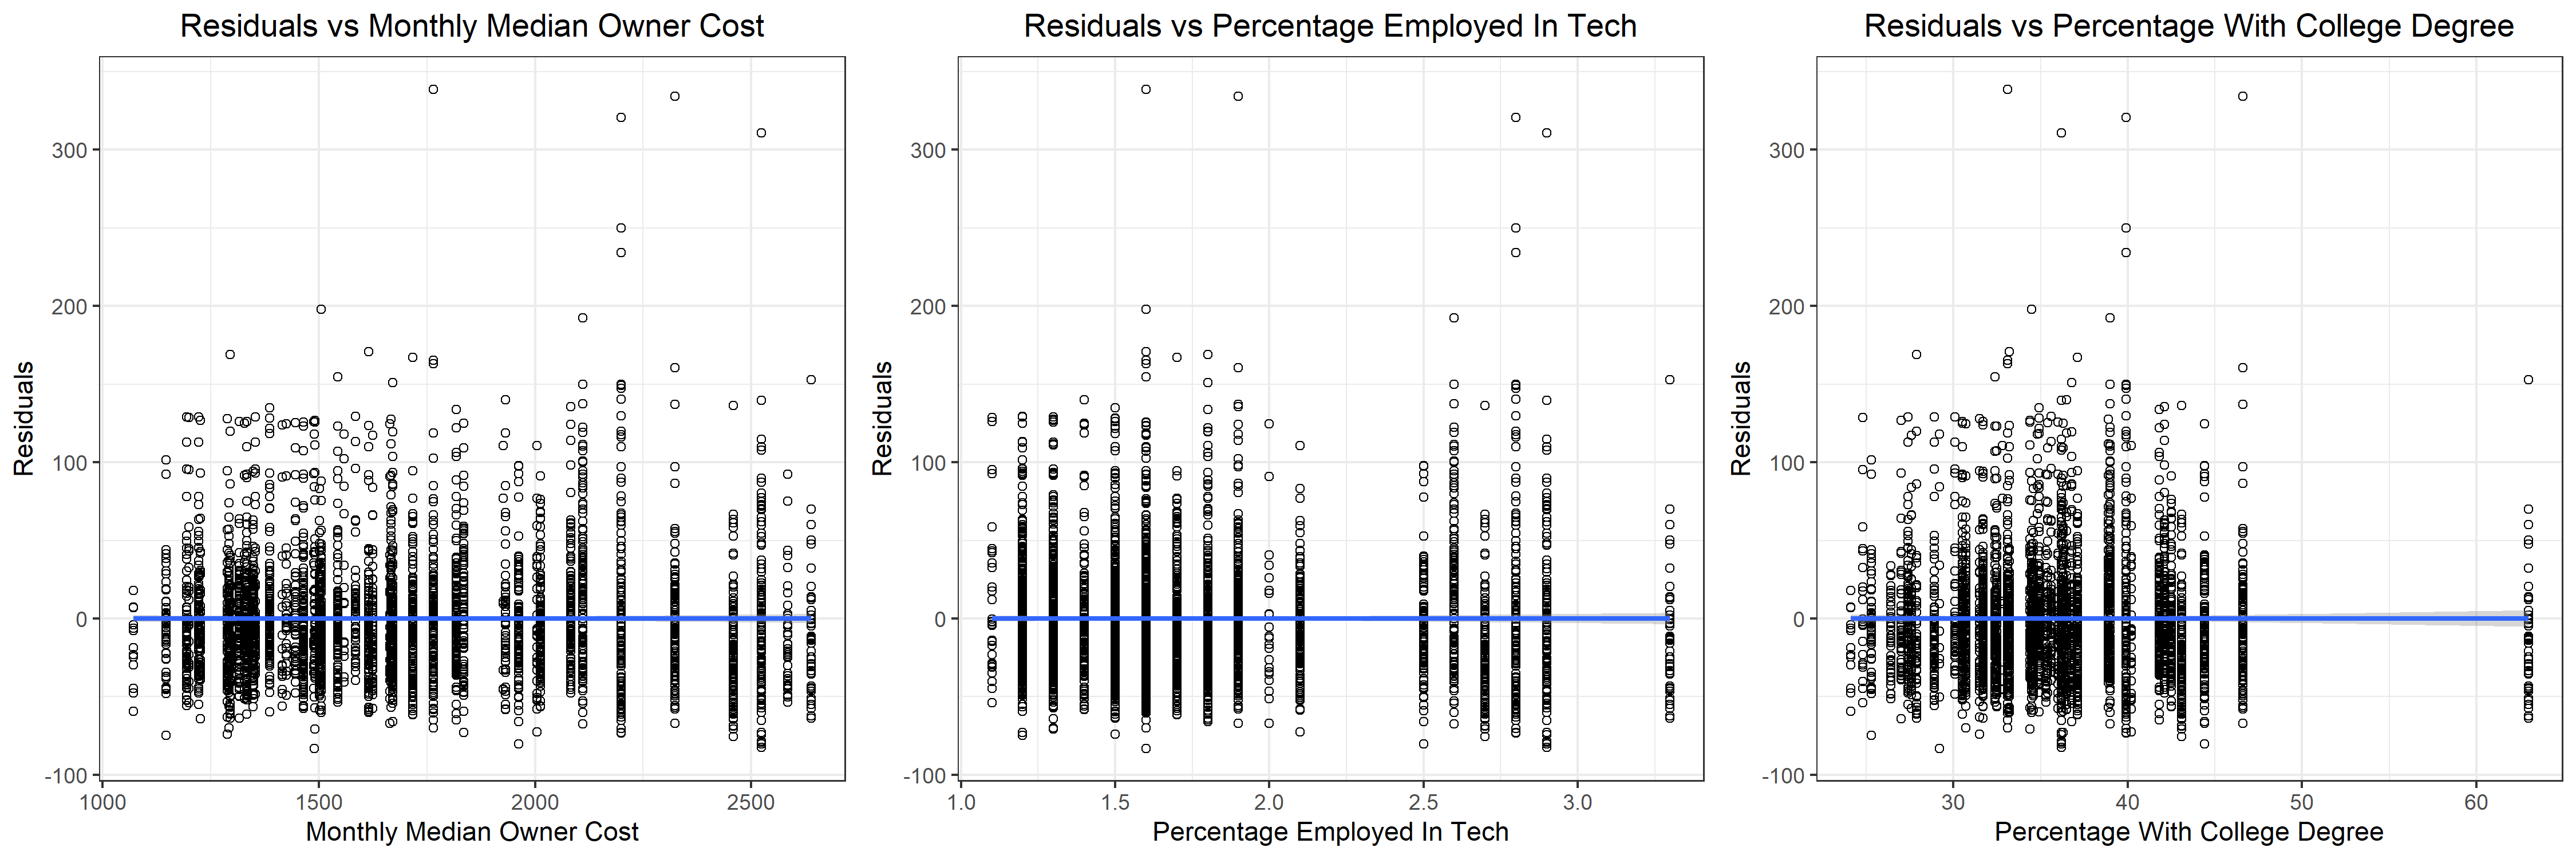
\includegraphics[width=\textwidth]{residuals_check1.png}
	\end{figure}

	\begin{figure}[h]
	\caption{Residuals from model in Table (2) Column (6)}
	\centering
	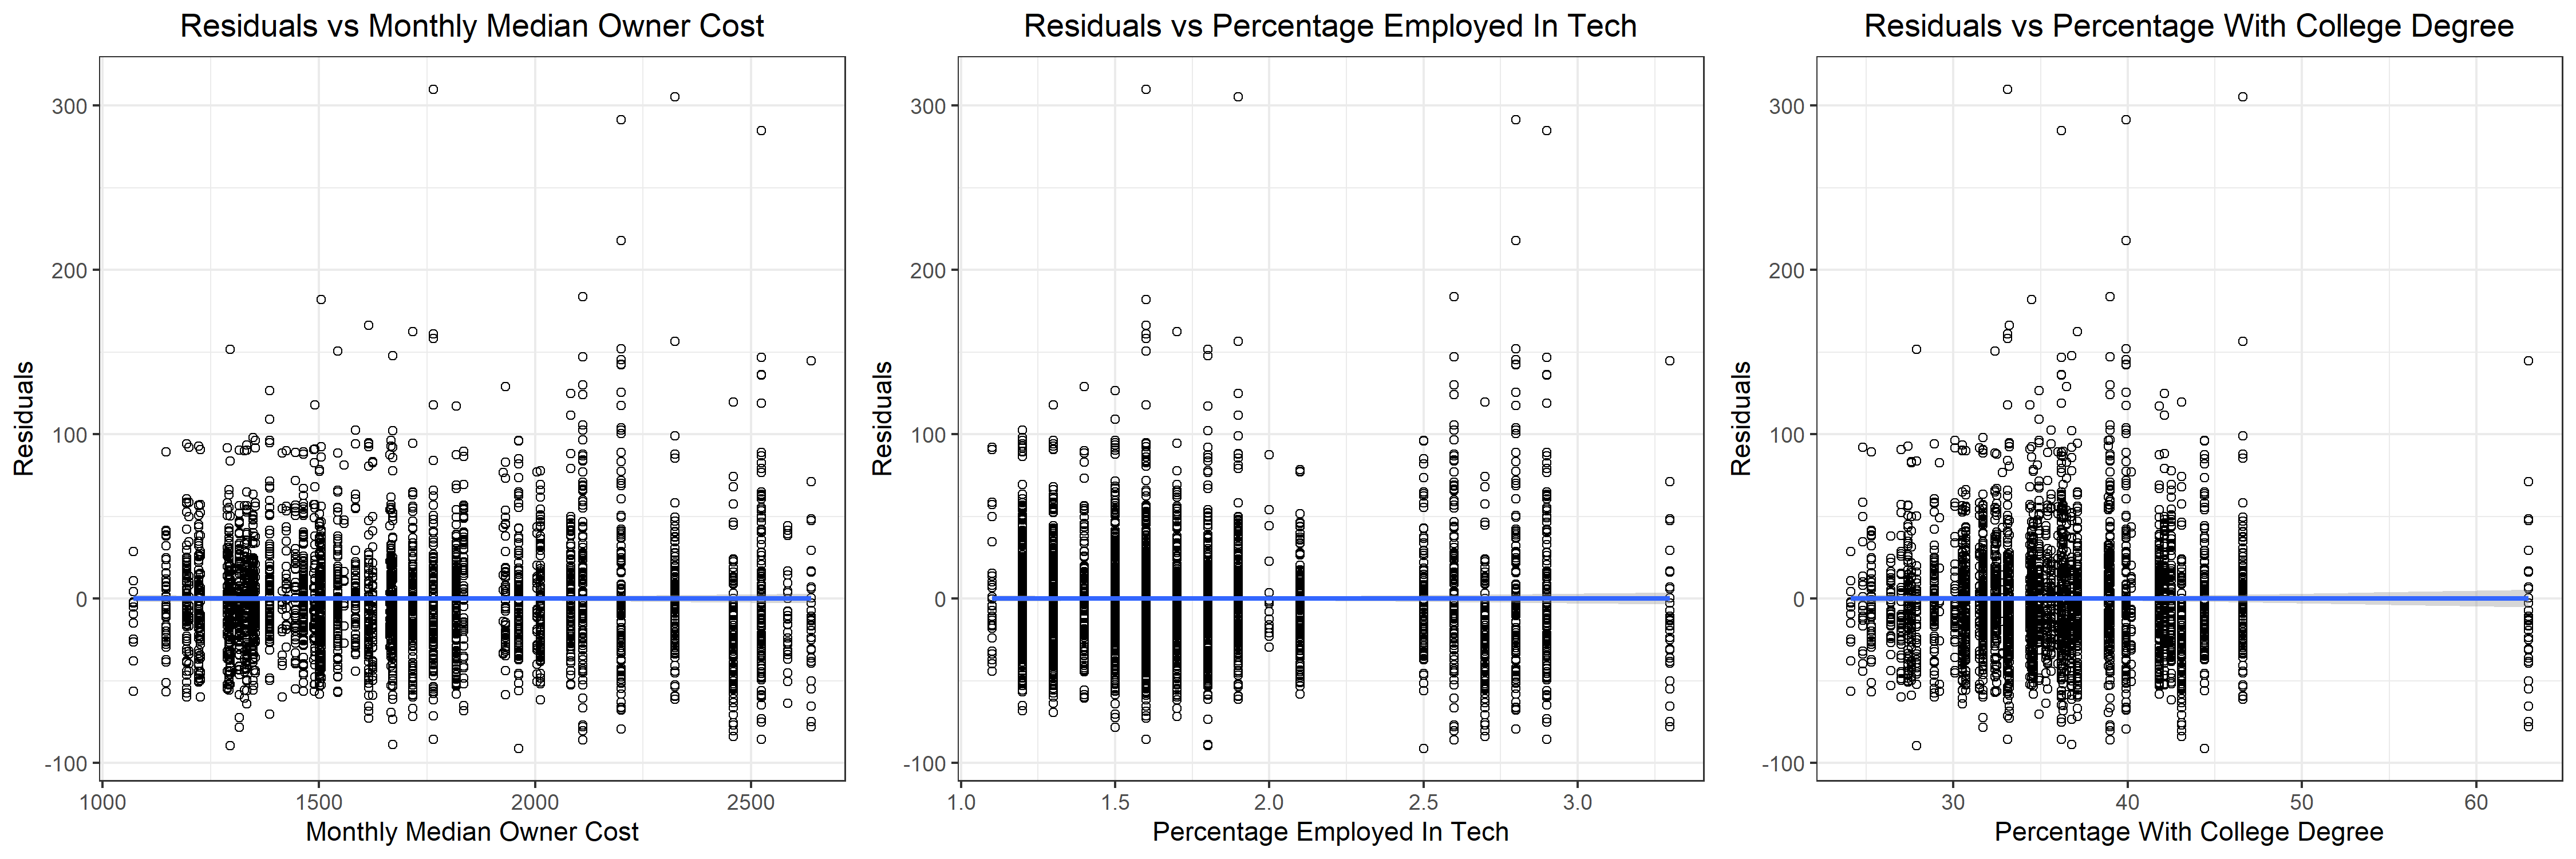
\includegraphics[width=\textwidth]{residuals_check2.png}
	\end{figure}

	\begin{figure}[h]
	\caption{Residuals from model in Table (3) Column (2)}
	\centering
	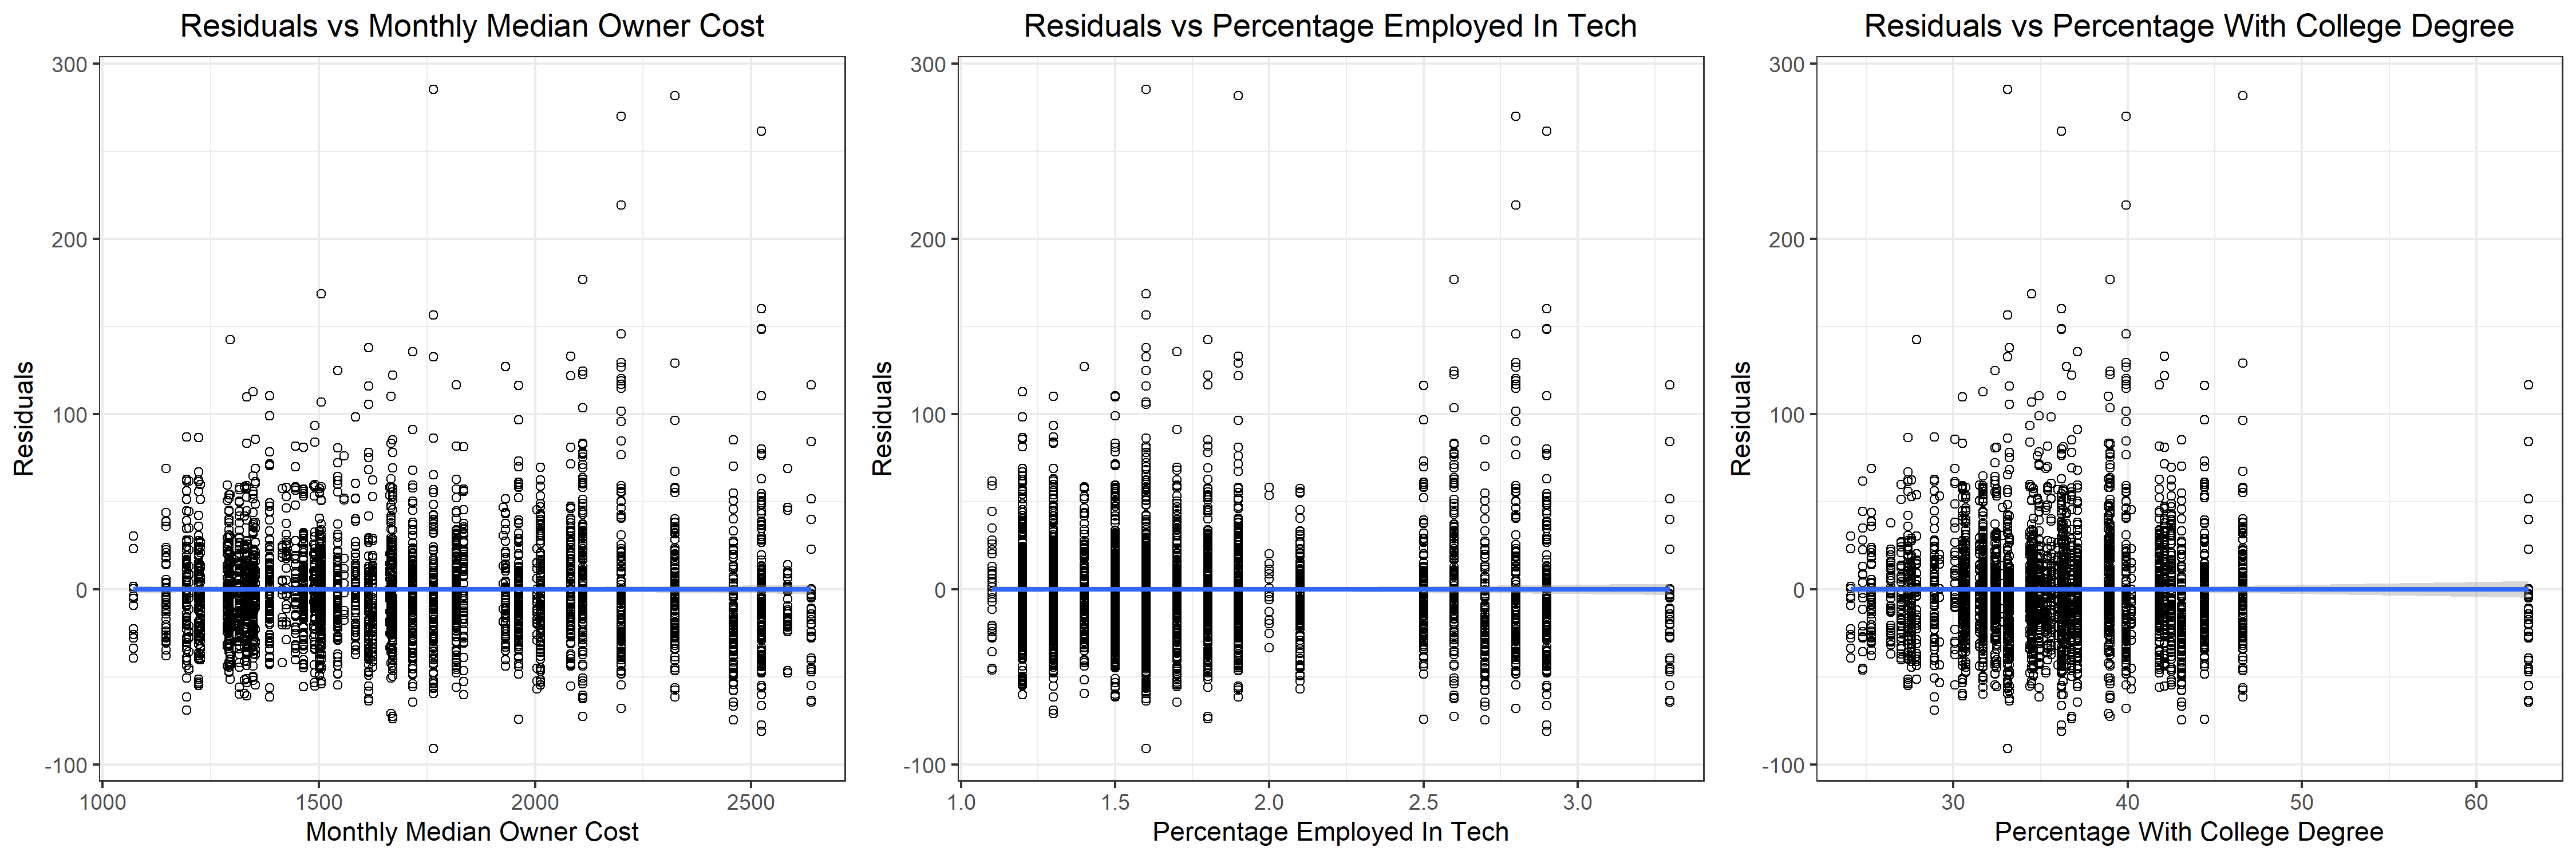
\includegraphics[width=\textwidth]{residuals_check3.png}
	\end{figure}

	\begin{figure}[h]
	\caption{Distribution of Residuals}
	\centering
	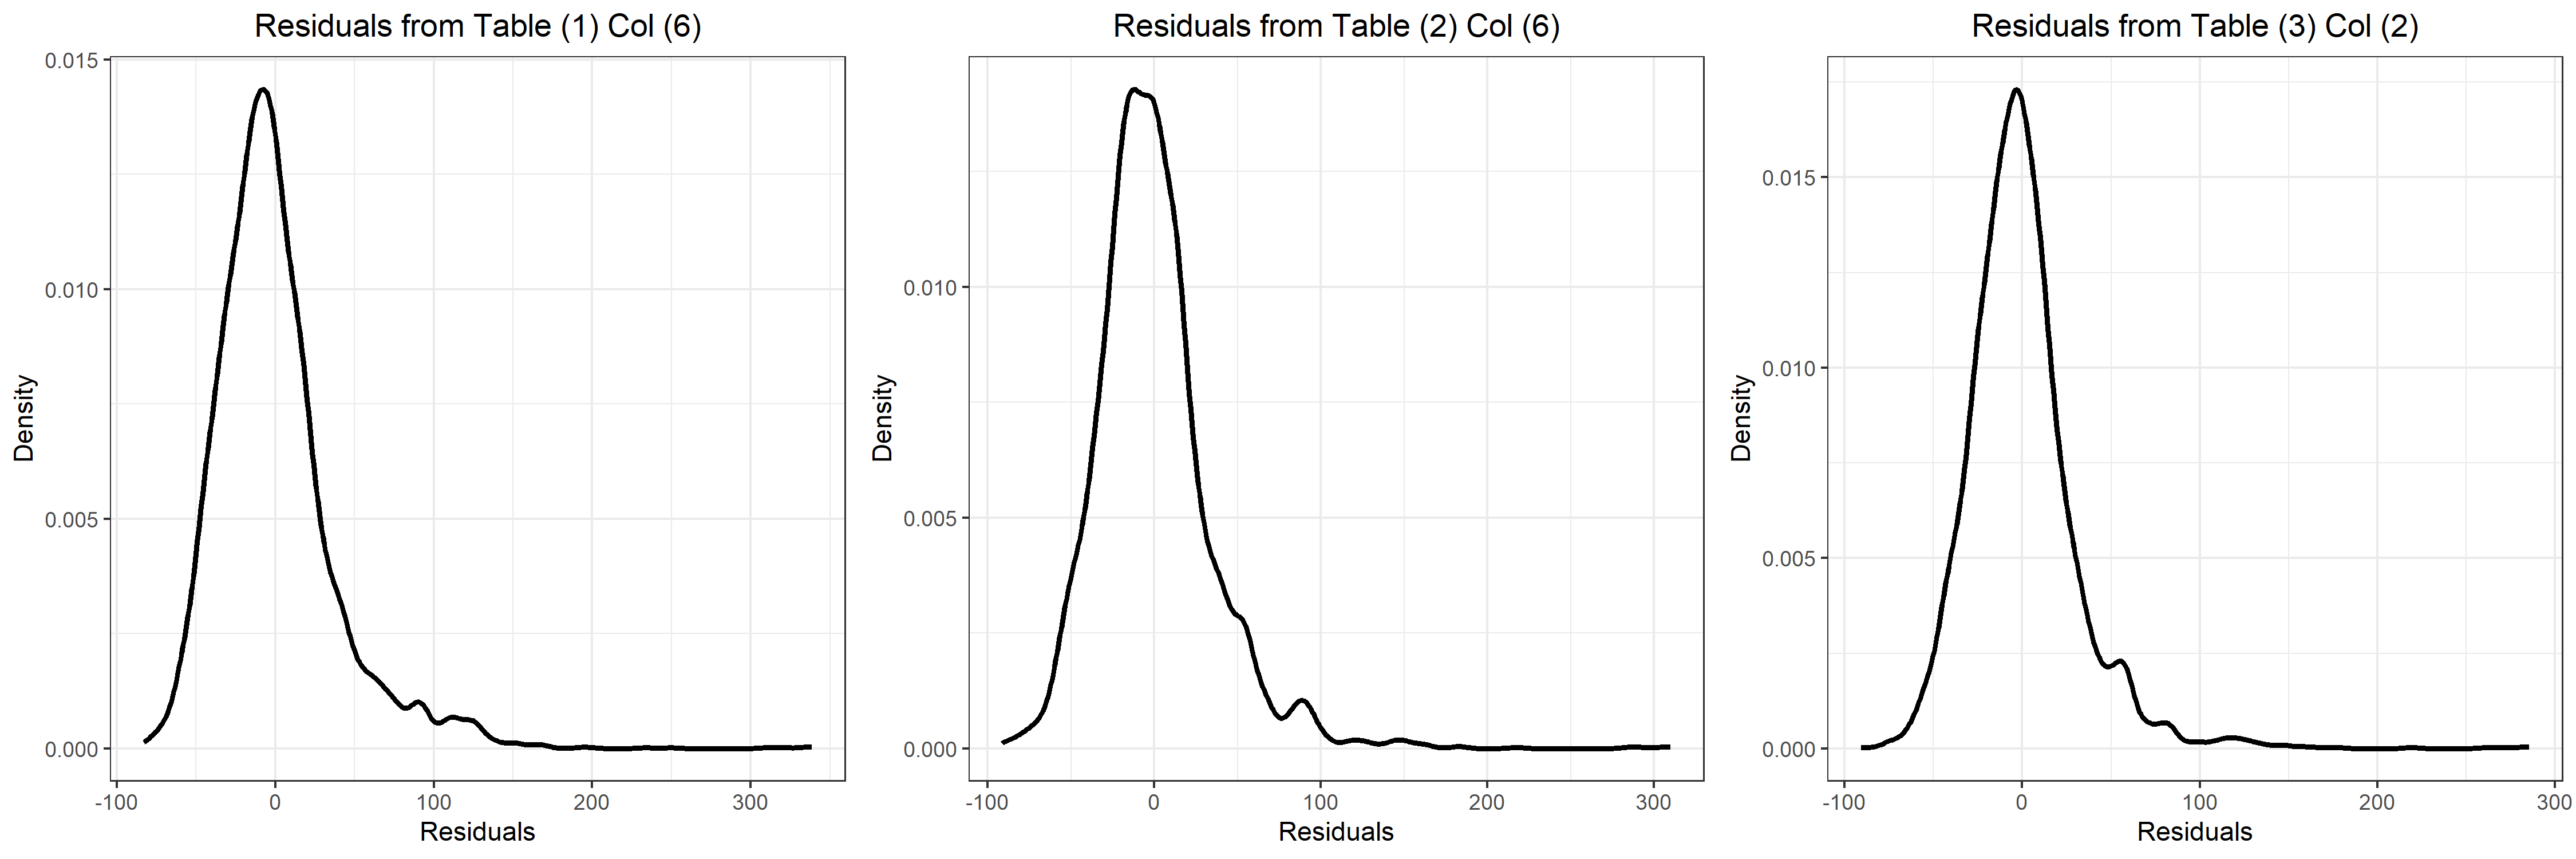
\includegraphics[width=\textwidth]{residuals_distribution.png}
	\end{figure}
	
\end{document}